\chapter{Service-Modelle des Cloud Computing}
\label{cha:service-modelle_des_cloud_computing}
Cloud-Services werden üblicherweise in ein Schichtenmodell eingeteilt. Man unterscheidet dabei drei Schichten:
\begin{enumerate}
      \itemsep0pt
      \item Software as a Service (SaaS)\cite{microsoft_cloud_2014-1}
      \item Platform as a Service (PaaS)\cite{microsoft_cloud_2014-2}
      \item Infrastructure as a Service (IaaS)\cite{microsoft_cloud_2014}
\end{enumerate}
Die Zuteilung eines Services zu einer Schicht erfolgt anhand der Ebene im IT-Stack auf der der Service angesiedelt ist.
Die drei Ebenen lassen sich in einer Pyramidenform darstellen. (siehe Abb \ref{fig:iaas_paas_saas}) 

\begin{figure}[htb]
  \centering  
  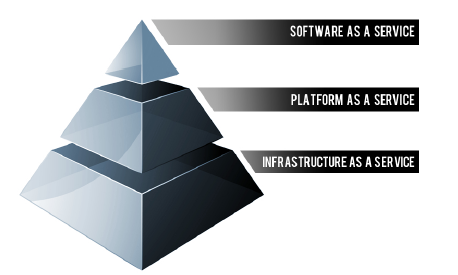
\includegraphics[scale=0.7]{img/iaas_paas_saas.png}\\
  \footnotesize\sffamily\textbf{Quelle:} \cite{kepes_understanding_2014}
  \caption{Cloud Computing Modelle}
  \label{fig:iaas_paas_saas}
\end{figure}

Die höheren, abstrakten Schichten nutzen dabei die Dienste der tieferen, konkreten Schichten.
Docker kann die Cloud-Services vor allem in der Schicht Platform as a Service unterstützen.
Im folgenden werden die einzelnen Schichten kurz näher erklärt.
\section{Infrastructure as a Service (IaaS)}
\label{sec:iaas}
Die unterste Schicht bildet die Infrastructure as a Service-Schicht.
\glqq Diese Schicht stellt Mittel bereit, mit denen Basisspeicher und Rechenleistung als standardisierte Services über das Netzwerk angeboten werden können.\grqq \cite[S. 30]{meinel_virtualisierung_2011}
Anstelle sich Server, Speicherplatz und Netzwerk selbst zu kaufen, können Nutzer diese Resourcen
bei Bedarf von einem Infrastructure as a Service-Provider beziehen. Die Wartung und Pflege der Hardware kann so entfallen.
Dem Nutzer von Infrastructure as a Service wird eine Plattform bereitgestellt, über die er volle Kontrolle hat. Diese Plattform ist dabei jederzeit skalierbar. Kurzzeitiger bedarf an zusätzlichen Hardwareressourcen kann so kostengünstig ausgeglichen werden und muss nicht durch überschüssige, ungenutzte Hardware abgesichert werden.
Schwierige Planungen über den erwarteten Bedarf an Ressourcen können so entfallen und das Risiko einer Fehlplanung eliminiert werden.

\section{Platform as a Service (PaaS)}
\label{sec:paas}
Die mittlere Schicht bezeichnet man als Platform as a Service. In diese Schicht fallen Services, die ein \glqq Programmiermodell und Entwicklungswerkzeuge bereitstellen, um Cloudbasierte Anwendungen zu erstellen und auszuführen.\grqq \cite{sommergut_faq_2014}
Der Nutzer von Platform as a Service soll in der Lage sein, seine Anwendung zu entwickelte und zu betreiben ohne sich dabei um die Rahmenbedingungen wie Hardware oder Software Infrastruktur kümmern zu müssen.
Der Platform as a Service-Provider liefert also alle nötigen Ressourcen wie Rechenleistung, Speicher und Netzwerk und skaliert diese abhängig von den Anforderungen der jeweiligen Anwendung.
Schwierige Aufgaben wie z.B. Loadbalancing werden dem Entwickler so abgenommen.
Platform as a Service setzt auf der darunterliegenden Schicht Infrastructure as a Service auf.
Auch bei Platform as a Service wird eine Infrastruktur bereitgestellt, diese wird aber noch um eine Ebene erweitert die es ermöglicht Webanwendungen schnell und einfach zu erstellen.

Unternehmen sind immer auf der Suche ihren Kunden einen besseren Service und Support zu liefern.
Dabei wird in der heutigen Zeit zumeist auf Webanwendungen gesetzt. Das Entwickeln und Betreiben dieser Anwendungen erweist sich allerdings oftmals als sehr zeitaufwendig und kostenintensiv.
Platform as a Service versucht dieses Problem zu lösen indem es den Entwicklern eine fertige Plattform anbietet. Die Entwickler können sich so ganz alleine auf die Entwicklung konzentrieren und müssen sich nicht um die gesamte Infrastruktur kümmern.

\section{Software as a Service (SaaS)}
\label{sec:saas}
Die höchste Schicht des Modells bildet die Anwendungsschicht, die sogenannte Software as a Service-Schicht.
Software as a Service ist analog zu Platform as a Service zu betrachten. Hierbei wird jedoch keine Plattform zum entwickeln von Software über das Internet bereitgestellt, sondern die Software selbst. \cite{kepes_understanding_2014}
Software as a Service ist der wohl bekannteste und am häufigsten genutzte Cloud-Service. Die Nachfrage nach Software die nach diesem Modell bereitgestellt wird hat sich in den letzten Jahren rasant entwickelt. Dies ist vor allem dem Komfort den Software as a Service bietet geschuldet.
Mit Software as a Service müssen sich Anwender nicht mehr mit ihrer eigen Hardware- und Softwareausstattung oder ihrem Betriebssystem auseinandersetzen wie sie es bisher gewohnt waren. Software wird ihnen einfach als Service über das Internet bereitgestellt.

Der Software as a Service \glqq Ansatz sieht vor, dass einzelne Softwarekomponenten bei einem Dienstleister betrieben werden, der allein für die gesamte Administration der Software verantwortlich ist, also Hardware und Software, Wartung und Betrieb. Dies betrifft auch die interne Ressourcenanpassung zur performanten Bereitstellung der Dienste.\grqq \cite[S. 34]{meinel_virtualisierung_2011}

Aus Unternehmenssicht werden dadurch Kosten gespart, da zeitaufwendige Aufgaben wie die Installation und Auslieferung der Software entfallen. Aufgaben wie das Aktualisieren veralteter Software werden vom Software as a Service-Provider übernommen. Dadurch, dass die Software nicht mehr selbst verwaltet werden muss, sind neue Features oft sofort verfügbar und nicht erst mit dem nächsten Update-Zyklus der Unternehmens.
Darüber hinaus werden Software as a Service-Produkte oftmals nach der tatsächlichen Nutzung abgerechnet. Das ermöglicht es Unternehmen neue Plattformen ohne eine langfristige Bindung zu testen oder nur kurzzeitig zu nutzen.